\documentclass{article}

\usepackage{amsmath,amssymb}
% \usepackage{fullpage}
\usepackage{enumerate}
\usepackage{hyperref}
\usepackage{graphicx}
\graphicspath{{../logos/}}


\begin{document} \thispagestyle{empty}

\setlength{\tabcolsep}{5pt}
\begin{center} \begin{tabular}{cccc}
	% set heights below to 43pt if fullpage not used
	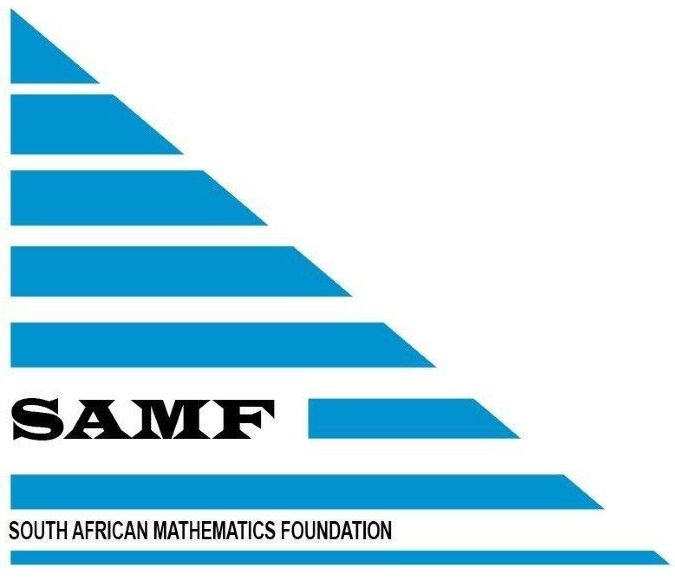
\includegraphics[height=43pt]{SAMF_logo.jpg} &
	
\includegraphics[height=43pt]{SAICA_logo.jpg} &
	
\includegraphics[height=43pt]{OM_Logo_Stacked_Vignette_on_White_RGB.jpg} &
	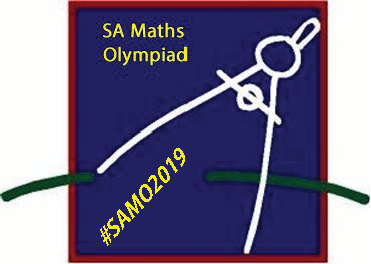
\includegraphics[height=43pt]{SAMO2019.png}
\end{tabular} \end{center}


\bigskip


\begin{center}
\textbf{\Large Intermediate February Monthly Problem Set}
\\ \vspace{1em}
\textbf{\large Due: 4 March 2020}
\end{center}


\begin{enumerate}

\bigskip
\item % Croatia 2014
On a $5 \times 7$ board all squares are coloured white. Exactly 17 squares need to be coloured black, so that the new arrangement of black and white squares is centrally symmetric, i.e. so that it does not change if it is rotated by $180^{\circ}$ around the centre of the board. In how many ways is it possible to do this?


\bigskip
\item % Croatia 2014
Find all positive integers $a,b,c,n$ such that $a!+b!+c! = 2^n$.


\bigskip
\item % Croatia 2014
Let $n$ be a positive integer and let $S$ be the sum of all integers from 1 to $n$. Prove that $S+1$ is not divisible by 3.


\bigskip
\item 
A chessboard is a board with 8 rows and 8 columns, whose squares are coloured alternately black and white, so that the square in the first row and first column is coloured black.
An integer is written in each square.
It is known that the sum of all the numbers on the white squares equals 26 and the sum of all the numbers in the odd rows equals 43.
If we change the sign of all the numbers on white squares, what will be the sum of all the numbers in the odd columns after the change?


\bigskip
\item % Croatia 2014
Let $ABCD$ be a parallelogram with acute angle at $A$.
Let $E$ be the foot of the perpendicular from $C$ to the line $AB$ and let $F$ be the foot of the perpendicular from $C$ to the line $AD$.
Prove that
\[ AB \cdot AE + AD \cdot AF = AC^2. \]


\smallskip
\item % Croatia 2014
Find all pairs of real numbers $(x,y)$ satisfying the following system:
\begin{align*}
x + y^2 &= y^3, \\
y + x^2 &= x^3.
\end{align*}
	

\medskip
\item % Malwande, G
Let $ABC$ be a triangle with orthocentre $H$, such that $AB<BC$ and $\angle BAC < 90^\circ$.
Let the circle $\Gamma$ centred at $B$ and passing through $A$ intersect $AC$ again at $D$.
The circumcircle of $\triangle BCD$ intersects $\Gamma$ again at $E$.
$ED$ and $BH$ intersect at $F$.
Prove that $BD$ is tangent to the circumcircle of $\triangle DHF$.


\medskip
\item % IMO Long List 1992 Q65, A
For any 4 points in $\mathbb{R}^3$, does there exist a plane such that the orthogonal projections of the points on the plane make up the vertices of a parallelogram?


\end{enumerate}


\vfill
\textbf{\Large Email submission guidelines}
\begin{itemize}
	\item Email your solutions to \href{mailto:samf.training.assignments@gmail.com}{\texttt{samf.training.assignments@gmail.com}}.
	\item In the subject of your email, include your name and the level of the assignment (Beginner, Intermediate or Senior).
	\item Submit each question in a single separate PDF file (with multiple pages if necessary), with your name and the question number written on each page.
	\item If you take photographs of your work, use a document scanner such as Office Lens to convert to PDF.
	\item If you have multiple PDF files for a question, combine them using software such as PDFsam.
\end{itemize}

\end{document}